\documentclass[tikz]{standalone}

\usepackage[latin1]{inputenc}
\usepackage{tikz,physics}
\usetikzlibrary{quotes,angles,calc,decorations.markings}
% GNUPL
% Draw line annotation
% Input:
%   #1 Line offset (optional)
%   #2 Line angle
%   #3 Line length
%   #5 Line label
% Example:
%   \lineann[1]{30}{2}{$L_1$}
\newcommand{\lineann}[4][0.5]{%
    \begin{scope}[rotate=#2, blue,inner sep=2pt]
        \draw[densely dashed, blue!40] (0,0) -- +(0,#1)
            node [coordinate, near end] (a) {};
        \draw[densely dashed, blue!40] (#3,0) -- +(0,#1)
            node [coordinate, near end] (b) {};
        \draw[|<->|] (a) -- node[fill=white] {#4} (b);
    \end{scope}
}
\begin{document}
\pagestyle{empty}


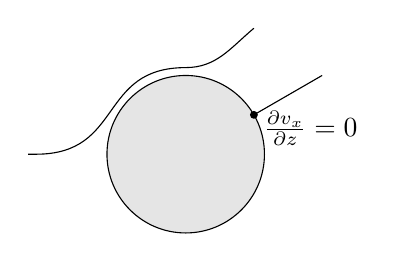
\begin{tikzpicture}[
    scale=1, 
    arrowline/.style={black},
    kos/.style={black},
    tangent/.style={
        decoration={
            markings,% switch on markings
            mark=
                at position #1
                with
                {
                    \coordinate (tangent point-\pgfkeysvalueof{/pgf/decoration/mark info/sequence number}) at (0pt,0pt);
                    \coordinate (tangent unit vector-\pgfkeysvalueof{/pgf/decoration/mark info/sequence number}) at (1,0pt);
                    \coordinate (tangent orthogonal unit vector-\pgfkeysvalueof{/pgf/decoration/mark info/sequence number}) at (0pt,1);
                }
        },
        postaction=decorate
    },
    use tangent/.style={
        shift=(tangent point-#1),
        x=(tangent unit vector-#1),
        y=(tangent orthogonal unit vector-#1)
    },
    use tangent/.default=1
    ]



    % \draw[arrowline] (0,0)  to [out=90,in=-90] node[sloped,pos=0.5]{\tikz{\draw[<-,arrowline](0,0) -- ++(0.1,0)}} ++(-0.5,1) to [out=90,in=-90] node[sloped,pos=0.5]{\tikz{\draw[->,arrowline](0,0) -- ++(0.1,0)}} ++ (0.5,1);

    % \draw[arrowline,rotate around={180:(0.5,1)}] (0,0)  to [out=90,in=-90] node[sloped,pos=0.5]{\tikz{\draw[<-,arrowline](0,0) -- ++(0.1,0)}} ++(-0.5,1) to [out=90,in=-90] node[sloped,pos=0.5]{\tikz{\draw[->,arrowline](0,0) -- ++(0.1,0)}} ++ (0.5,1);

    % \draw[arrowline] (0.5,0)  -- node[sloped,pos=0.8]{\tikz{\draw[->,arrowline](0,0) -- ++(0.1,0)}} ++(0,2);

    % \begin{scope}[xshift=0.5cm,yshift=1cm]
    %     \draw[->,>=latex] (0.5,0) -- ++(-0.45,0);
    %     \draw[->,>=latex] (-0.5,0) -- ++(0.45,0);
        \draw[fill=black!10] (0,0) circle (1);

        \draw[fill=black] (30:1) circle (1.2pt) node[right,yshift=-0.5em] {$\pdv{v_x}{z}=0$} -- (30:2);
    %     \draw[fill,black!30] (-0.5,0) circle (0.25);
    % \end{scope}

    \draw[] (-2,0) -- (-1.9,0)  to [out=0,in=180,looseness=1.3]  (0,1.1) to[out=0,in=220] ++(30:1);

    % \draw [use tangent=1,->,kos] (0,0) -- (0.75,0) node[right] {$\vec{v}$};
    % \draw [use tangent=2,->,kos] (0,0) -- (0.75,0) node[right] {$\vec{v}$};
    % \draw[tangent=0.79,arrowline] (0,0)  to [out=0,in=120] node[sloped,pos=0.5]{\tikz{\draw[->,arrowline](0,0) -- ++(0.1,0)}} (3,0);
    % \draw [use tangent,->,kos] (0,0) -- (0.75,0) node[right] {$\vec{v}$};

\end{tikzpicture}


\end{document}